% ==============
% PARAMETRAGES
% à compiler en pdfLaTeX
% ==============

% GENERAL
%  type de document rapport, chapitre commence en page impaire ou paire indifféremment
\documentclass[twoside,a4paper,11pt,frenchb,openany]{report}  
%  type de document, chapitre commence en page impaire
%\documentclass[twoside,a4paper,12pt,frenchb,openright]{report} 
\title{\textbf{Rapport de stage \\ Publication du package crisprbuilder\_tb}}
\author{Stephane Robin sous la direction de Christophe Guyeux et Jean-Claude Charr}
\date{\today}

% IMPORTATION DE LIBRAIRIES
\usepackage{amssymb}  % symboles
\usepackage{amsmath}  % symboles mathématiques
\usepackage{amsfonts}  % polices de caractères
\usepackage{amscd}
\usepackage{amsthm}  % symboles mathématiques pour redéfinir les théorèmes
\usepackage[all,cmtip]{xy}
\usepackage{array}  % tableaux
\usepackage[frenchb]{babel}  % langue française
\usepackage{bm}  % caractères grecs
\usepackage{calc}
\usepackage[justification=centering]{caption} % centralise les légendes des figures
\usepackage{enumitem} % listes
\usepackage{eurosym}  % symbole euro
\usepackage{euscript}
\usepackage{fancybox}  % boîtes
\usepackage{float}  % images flottantes
\usepackage[T1]{fontenc}  % LaTeX modele
\usepackage[top=3.1cm,bottom=2.7cm,left=2.2cm,right=2.2cm,dvips]{geometry}  % marges
\usepackage{graphicx}  % insertion images
\usepackage{imakeidx} % make index
\usepackage[utf8]{inputenc}  % accents
\usepackage{mathrsfs}  % symboles mathématiques
\usepackage{mathtools}  % outils mathématiques
\usepackage{mdframed} % box autour des theoremes
\usepackage{pst-plot, pstricks}
\usepackage{pstricks-add}
\usepackage{rotating}
\usepackage{setspace} % permet de définir l'espace entre les lignes
\usepackage{srcltx}
\usepackage[most]{tcolorbox}
\usepackage{textcomp}   % caracteres complementaires
\usepackage{titlesec}  % sections
\usepackage{titletoc}  % table de contents
%\usepackage[nottoc,notlof,notlot]{tocbibind}  % bibliothèque
\usepackage{verbatim}  % caracteres non interpretes
\usepackage{wrapfig}  % pour inserer les figures dans du texte

% COULEURS
\definecolor{couleurTitre}{RGB}{64,128,128}  % doit être défini avant xcolor
\definecolor{couleurUrl}{RGB}{127,62,0}
\usepackage{xcolor}  % couleurs
%\definecolor{amber}{rgb}{1.0,0.49,0.0} % couleur non utilisee
%\definecolor{greyish}{rgb}{52.0,160.0,157.0} % couleur non utilisee
%\definecolor{theoremeCouleur}{rgb}{224.0,90.0,67.0} % couleur non utilisee

% LISTES
\renewcommand{\labelitemi}{$\bullet$}  % symboles de listes
\frenchbsetup{StandardLists=true}  % style de bullets

% IMAGES
\usepackage{caption}  % insertion d'images
\usepackage[font=footnotesize,labelfont=bf]{caption}  % légendes des images
\renewcommand{\thefigure}{\arabic{figure}}  % numérotation des images
%\renewcommand{\thefigure}{\arabic{section}.\arabic{figure}}  % autre possibilité numérotation des images
\usepackage{subcaption}

% HYPERLINKS
\usepackage{hyperref}
\hypersetup{
	colorlinks=true,
	linkcolor=couleurUrl,
	citecolor=couleurUrl,
	urlcolor=couleurUrl,
	breaklinks=true % saute la ligne au milieu d'un href
}
\PassOptionsToPackage{hyphens}{url}\usepackage{hyperref} % pour que url ait les memes propriétés que hyperref

% LIGNES
\usepackage{parskip}
%\setlength\parskip{\baselineskip} % joint a la suppression de l'espace horizontal
%\setlength{\parindent}{0cm} % supprime l'espace horizontal en debut de ligne

% HEADINGS AND FOOTERS
\usepackage{fancyhdr}  % entete
\pagestyle{fancy}  % la page accepte les entetes et pieds de page
\renewcommand{\headrulewidth}{0pt}
\fancyhead[L,R,C]{}
%\fancyhead[LE]{} % pages paires header gauche
%\fancyhead[CE]{} % pages paires header centre
%\fancyhead[RE]{Le théorème de Pythagore} % pages paires header droit
%\fancyhead[LO]{Le théorème de Pythagore} % pages impaires header gauche
%\fancyhead[CO]{} % pages impaires header centre
%\fancyhead[RO]{} % pages impaires header droit
%\fancyfoot[c]{\textcolor{gray}{\thepage}}  % pied de page
%\fancyfoot[L,R,C]{} % forcing footer empty

% REDEFINITION DU STYLE DE THEOREM
\newmdtheoremenv[  % definitions
linewidth=5,
leftline=true,
rightline=false,
bottomline=false,
topline=false,
leftmargin=0,
rightmargin=0,
backgroundcolor=couleurTitre!20,
linecolor=orange!70,
innertopmargin=21pt,
skipabove=\topskip,
ntheorem=true]{definition}{Définition}

\newmdtheoremenv[  % theoremes
linewidth=5,
leftline=true,
rightline=false,
bottomline=false,
topline=false,
leftmargin=0,
rightmargin=0,
backgroundcolor=couleurTitre!20,
linecolor=orange!70,
innertopmargin=10pt,
skipabove=\topskip,
ntheorem=true]{theorem}{}

\newmdtheoremenv[  % proprietes
linewidth=5,
leftline=true,
rightline=false,
bottomline=false,
topline=false,
leftmargin=0,
rightmargin=0,
backgroundcolor=couleurTitre!20,
linecolor=orange!70,
innertopmargin=21pt,
skipabove=\topskip,
ntheorem=true]{property}{Propriété}

\newmdtheoremenv[  % propositions
linewidth=5,
leftline=true,
rightline=false,
bottomline=false,
topline=false,
leftmargin=0,
rightmargin=0,
backgroundcolor=couleurTitre!20,
linecolor=couleurTitre!70,
innertopmargin=21pt,
skipabove=\topskip,
ntheorem=true]{proposition}{Proposition}

\newmdtheoremenv[  % corollaires
linewidth=5,
leftline=true,
rightline=false,
bottomline=false,
topline=false,
leftmargin=0,
rightmargin=0,
backgroundcolor=couleurTitre!20,
linecolor=couleurTitre!70,
innertopmargin=21pt,
skipabove=\topskip,
ntheorem=true]{corollary}{Corollaire}

\newmdtheoremenv[  % lemmes
linewidth=5,
leftline=true,
rightline=false,
bottomline=false,
topline=false,
leftmargin=0,
rightmargin=0,
backgroundcolor=couleurTitre!20,
linecolor=couleurTitre!70,
innertopmargin=21pt,
skipabove=\topskip,
ntheorem=true]{lemma}{Lemme}

% BOXES
\tcbset{
    frame code={}
    center title,
    left=0pt,
    right=0pt,
    top=0pt,
    bottom=0pt,
    colback=gray!40,
    colframe=white,
    width=\dimexpr\textwidth\relax,
    enlarge left by=0mm,
    boxsep=5pt,
    arc=0pt,outer arc=0pt,
    }


% NUMEROTATION DES CHAPITRES-SECTIONS
\renewcommand{\theequation}{\arabic{chapter}.\arabic{equation}}  % equations
%\renewcommand{\theequation}{\thesection\arabic{equation}}  % equations
%\numberwithin{equation}{section}  % equations

%\renewcommand{\thepart}{\Alph{part}}  % parties
%\renewcommand{\thechapter}{\arabic{chapter}.}  % chapitres
\renewcommand{\thesection}{\arabic{section}.}  % sections
\renewcommand{\thesubsection}{\arabic{section}.\arabic{subsection}.}  %  sous-sections
\renewcommand{\thesubsubsection}{\arabic{section}.\arabic{subsection}.\arabic{subsubsection}.}  % sous-sous-sections

\renewcommand{\thedefinition}{\arabic{chapter}.\arabic{definition}}  % definitions
\renewcommand{\theorem}{}  % theoremes
\renewcommand{\theproperty}{\arabic{chapter}.\arabic{property}}  % property
\renewcommand{\theproposition}{\arabic{chapter}.\arabic{proposition}}  % propositions
\renewcommand{\thecorollary}{\arabic{chapter}.\arabic{corollary}}  % corollaires
\renewcommand{\thelemma}{\arabic{chapter}.\arabic{lemma}}  % lemmes
\setcounter{secnumdepth}{4}  % profondeur de numérotation

% FORMAT DES SECTIONS-TITRES
\titleformat{\section}{\normalfont\normalsize\bfseries}{\textcolor{couleurTitre}{\thesection}}{1.2em}
{\normalfont\large\bfseries\scshape\textcolor{couleurTitre}} % format de titre de section
\titleformat{\subsection}{\normalfont\normalsize\bfseries}{\textcolor{couleurTitre}{\thesubsection}}{1em}
{\normalfont\normalsize\bfseries\textcolor{couleurTitre}}  % format de titre de sous-section
\titleformat{\subsubsection}{\normalfont\normalsize\bfseries\itshape}{\textcolor{couleurTitre}{\thesubsubsection}}{1em}
{\normalfont\normalsize\bfseries\itshape\textcolor{couleurTitre}}  % format de titre de sous-sous-section

\makeatletter

% CONCERNE LA TABLE DES MATIERES
%\renewcommand{\@chapapp}{}  % le mot `chapitre'' n'apparait plus en titre de chapitre
\renewcommand\l@section{\@dottedtocline{1}{0em}{1.5em}}  % espacement dans le titre d'une section
\renewcommand\l@subsection{\@dottedtocline{1}{2.5em}{2.5em}}  % espacement dans le titre d'une sous-section
\renewcommand\l@subsubsection{\@dottedtocline{1}{5em}{2.5em}}  % espacement dans le titre d'une sous-sous-section

\makeatother
\makeindex

% ==============
% DEBUT DU DOCUMENT
% ==============

\begin{document}
	
\maketitle
	

	
% REMERCIEMENTS ----------------------------
	
\chapter*{Remerciements}
	
Je tiens à exprimer mes plus sincères remerciements à Messieurs Christophe Guyeux et Jean-Claude Charr, professeurs à l'université de Franche Comté pour m'avoir guidé, conseillé et soutenu durant le déroulement de ce stage. Leurs explcations et leur disponibilité malgré un emploi du temps chargé ont largement contribué à ma compréhension du sujet.

Je voudrais également souligner la patience dont ils ont fait preuve pour m'expliquer les notions de bioinformatique que j'ai été amené à découvrir durant ce projet. Il en ressort que j'ai particulièrement apprécié de travailler sous leur direction.



\tableofcontents



% PREAMBULE --------------------------
\chapter*{Préambule}



% PRESENTATION DU PROJET --------------------------------	
\section{Présentation du projet}

Christophe Guyeux, Jean-Claude Charr, ... ont créé du code "brut" leur permettant à la fois d'afficher et de stocker des données relatives à un SRA particulier. Ce code doit être rassemblé, réorganisé, nettoyé pour être conforme aux critères PEP. Il doit être rendu plus efficace si possible, et testé. Il doit s'exécuter en utilisant un CLI, et doit finalement être empaqueté pour qu'un utilisateur puisse l'utiliser quelque soit sa plateforme (Linux, MacOS ou Windows) une fois installé. Pour cela, il est nécessaire de publier ce package sur PyPI et de le documenter clairement en anglais pour en faciliter l'utilisation.

Notons qu'à terme, l'objectif du package sera de proposer une reconstitution du crispr.

Lorsque nous avons défini les objectifs du stage, il est immédiatement ressorti l'importance de lui donner un caractère pratique, qui pourrait être transposable dans le milieu professionnel. La reconstruction du programme à partir d'éléments de code, la nécessité de créer localement un environnement spécifique de travail et d'installer automatiquement cet environnement sur les ordinateurs des utilisateurs, la possibilité de faire fonctionner le package sur différentes plateformes, les différents tests effectués, la création et publication du package sont autant de compétences pratiques utiles, auxquelles il faut se confronter pour bien en comprendre les difficultés.



% NOTATIONS -------------------------
\section{Notations}

Définissons tout d'abord le vocabulaire que nous allons utiliser dans ce rapport de stage :
\begin{itemize}
\item module : un fichier contenant du code Python,
\item package : un répertoire contenant des modules Python,
\item distribution : une archive de modules ou packages (au format tar, whl, ...)
\end{itemize}



% ETAT DE L'ART -------------------------------------
\chapter{Etat de l'art}


	

% CHOIX DES OUTILS -----------------------------
\chapter{Le choix des outils}




% CHOIX DE L'ENVIRONNEMENT DE TRAVAIL -----------------------------
\section{L'environnement de développement}

 XXX -> CONSTRUCTION D'UN ENVIRONNEMENT DE TRAVAIL

Afin de tester les codes de ce projet, l'outil de création d'environnement virtuel \textit{venv} \index{venv} nous permet de créer un environnement de développement. \textit{venv} commence par constituer un dossier contenant tous les exécutables nécessaires à l'utilisation des modules d'un projet Python.

Il convient de définir la version de Python utilisée dans cet environnement de développement. Pour cela, le module \textit{pyenv} \index{pyenv} nous permet de définir une version de Python comme version locale de travail dans l'environnement. Nous choisissons pour les besoins du test Python 3.6.5.

Finalement, nous installons dans cet environnement les dépendances nécessaires à l'aide de l'outil \textit{pip} \index{pip} :
\begin{itemize}
\item pkg-resources==0.0.0 (installé automatiquement)
\item \begin{tcolorbox}\texttt{pip install xmltodict}\end{tcolorbox}
le module xmltodict permet de lire du code XML comme si il s'agissait de code JSON. Il permet donc une lecture plus rapide des fichiers.
\item  \begin{tcolorbox}\texttt{pip install openpyxl}\end{tcolorbox}
le package openpyxl permet de lire et d'écrire dans des fichiers Excel de type xlsx, xlsm, xltx, xltm. Il comprend les modules et-xmlfile et jdcal.
\item  \begin{tcolorbox}\texttt{pip install xlrd}\end{tcolorbox}
le module xlrd extrait des données d'un tableur Excel à partir de la version 2.0 et avant de les formatte.
\item  \begin{tcolorbox}\texttt{pip install biopython}\end{tcolorbox}
le package biopython regroupe un ensemble d'outils Python pour le traitement informatique de la biologie moléculaire et comprend le module numpy.
\item DateTime==4.3\\
Le module datetime permet de manipuler des dates et heures en gérant des objets de type DateTime. 
\item pytz==2019.3 (installé avec le module datetime)
\item zope.interface==5.0.1 (installé avec le module datetime)
\end{itemize}

Notons que certains modules utilisés dans ce package sont nativement présents dans Python3. C'est le cas par exemple de :
\begin{itemize}
\item le module os fournit une manière portable d'utiliser les fonctionnalités dépendantes du système d'exploitation,
\item le module pickle permet de sérialiser et désérialiser une structure d'objet Python. Il remplace le module primitif marshal. pickle se trouve déjà dans la librairie standard Python3,
\item le module csv implémente des classes pour lire et écrire des données liées à des feuilles de calcul ou des bases de données au format csv,
\item le module shutil propose des opérations sur les fichiers et collections de fichiers, notamment la copie et suppression de fichiers.
Le module subprocess.run permet de gérer de nouveaux processus, de se connecter à leurs flux d'input/output/erreurs. Il remplace plusieurs modules dépréciés : os. system, os.spawn*, os.popen*, popen2.*, commands.* 
\end{itemize}

Le package, une fois installé par l'utilisateur, devra fournir automatiquement un environnement de travail similaire, afin que son exécution soit rendue possible. On devra donc retrouver les modules installés via \textit{pip} dans un fichier tel que requirements.txt.
 

% COMPOSITION D'UN PACKAGE STANDARD ------------------
\section{Composition d'un package standard}

Un package standard comporte obligatoirement un fichier \textit{\_\_init\_\_.py} qui va définir la version du projet et le nom du module de lancement du programme (souvent \textit{\_\_main\_\_.py}). Il est toutefois acceptable et parfois même recommandé de conserver un fichier \textit{\_\_init\_\_.py} vide. 

Les fichiers \textit{setup.py},  \textit{requirements.txt}, \textit{LICENSE},  \textit{README.md} ET \textit{MANIFEST.in} sont également nécessaires.  
\begin{itemize}
\item \textit{setup.py} est le script de construction et configuration destiné au \textit{setuptools}. Il définit notamment le nom et la version du package, ainsi que les fichiers qu'il contient. Il sert également d'interface en ligne de commande relative aux différentes fonctionnalités du package. \textit{setup.cfg} est un fichier d'initialisation qui contient les options par défaut des commandes du \textit{setup.py}.
\item \textit{requirements.txt} permet l'installation des dépendances à l'aide d'un unique fichier contenant un module à installer par ligne. Il nécessite l'instruction 
\begin{tcolorbox}\texttt{pip install -r requirements.txt}\end{tcolorbox}
pour commencer ces installations.
\item \textit{LICENSE} définit les termes légaux de la distribution. De nombreux pays n'autorisent pas l'utilisation ou la distribution de packages qui ne disposent pas de licence.
\item \textit{README.md} décrit l'objectif du package, son installation, la nature de ses dépendances et les principales fonctionnalités.
\item \textit{MANIFEST.in} permet d'inclure dans le package certains fichiers qui ne sont pas automatiquement intégrés. 
\end{itemize}

L'ensemble des modules nécessaires au fonctionnement du package sont regroupés dans un répertoire portant le même nom que le package avec le fichier \textit{\_\_init\_\_.py}.

Avec la PEP-518, le PyPA a proposé un nouveau standard au format package.toml, qui remplace les fichiers setup.py, requirements.txt, setup.cfg, MANIFEST.in et Pipfile. C'est ce nouveau standard qui est utilisé lors de la création d'un package avec Poetry.

La commande poetry new nomPaquet permet de générer le squelette de l'application, comprenant les tests unitaires, le fichier pyproject.toml, le fichier README.rst que nous changeons au format markdown README.md, le répertoire du projet et le fichier init.py. Nous rajoutons un fichier LICENSE, les composants principaux de la librairie, le présent rapport de stage et un fichier .gitignore pour la gestion des versions.
	
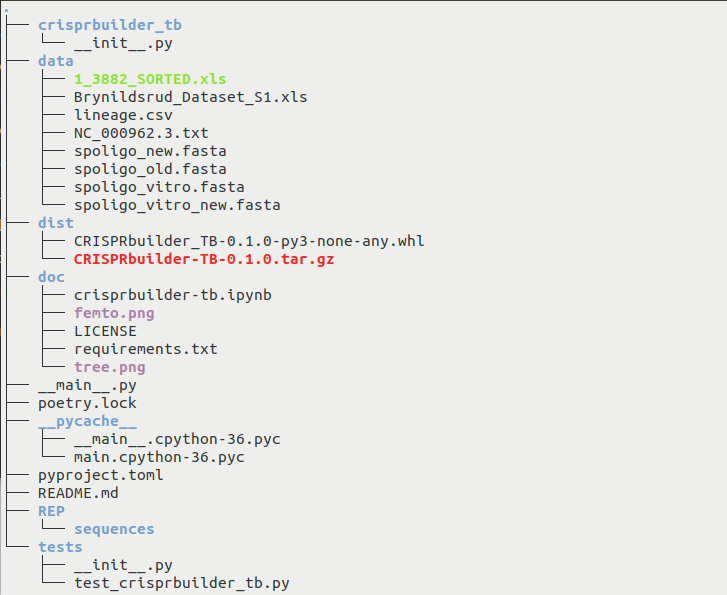
\includegraphics[width=9cm]{package_tree.png}

	La plupart des systèmes d'exploitation incorporent Python2.7 par défaut. L'environnement de travail devra donc expressément définir Python3 comme version pour le projet. Nous avons choisi la version 3.6.5 de Python dans le fichier package\_mymtc.toml.

Les paquets construits pour des systèmes Unix (Linux et MacOS) nécessitent l'incorporation de fichiers build.sh et meta.yaml. Les paquets construits pour les systèmes Windows nécessitent l'incorporation des fichiers bld.bat et meta.yaml. A VERIFIER DANS LE CAS DE POETRY


% QUELLE LICENCE CHOISIR ------------------
\subsection{Quelle licence choisir ?}
	
Trois licences retiennent notre attention. En voici les principales caractéristiques :
\begin{itemize}
\item	la licence MIT, courte et permissive, préserve exclusivement le copyright et les avis de licence. Toute modification ultérieure peut être distribuée suivant une licence différente et notamment utilisée à des fins personnelles ou commerciales, sans obligation de publication des codes source,
\item	la licence Apache (2.0) est également permissive et sensiblement similaire dans ses conditions à la licence MIT. Toutefois, elle requiert de préciser les modifications effectuées lors de nouvelles distributions,
\item	la licence GNU (GPL v3.0) préserve également le copyright et les avis de licence. Elle peut être utilisée à des fins personnelles et commerciales. Elle impose en outre, en cas de modification, la publication complète des codes et l'utilisation de la licence GNU pour les nouvelles distributions.
\end{itemize}

Dans le cadre de ce projet, aucune spécification restrictive n'étant requise, nous avons choisi la licence MIT qui est simple et peu contraignante.

	

% CHOIX DE L'OUTIL D'EMPAQUETAGE --------------------
\subsection{Choix de l'outil d'empaquetage}
	
	Le PyPA \textit{Python Packaging User Guide} recommande l'utilisation de :
\begin{itemize}
\item \textit{setuptools} pour définir des projets et créer des sources de distribution,
\item \textit{pipenv} pour la gestion des dépendances de packages lors du développement d'applications,
\item \textit{venv} pour isoler les dépendances particulières d'une application et créer un environnement de travail,
\item \textit{conda} permettant de fournir un environnement de travail favorable aux projets scientifiques, avec notamment tous les modules essentiels pré-installés,
\item \textit{buildout} pour les projets de développement Web,
\item \textit{poetry} pour un besoin particulier non couvert par \textit{pipenv},
\item \textit{pip} pour l'installation de librairies à partir de PyPI \textit{Python Package Index}.
\end{itemize}

Au regard de ces recommandations, nous avons testé les outils suivants dans le but de définir un environnement de développement et de construire un package incorporant les dépendances requises.

\textit{pipenv} est un gestionnaire de haut niveau pour les environnements, les dépendances et les packages Python. Contrairement à \textit{virtualenv}, \textit{pipenv} distingue les dépendances du projet et les dépendances des dépendances du projet. Par ailleurs, \textit{pipenv} différencie le mode développement du mode production. Il offre l'avantage de bien fonctionner sur Windows. Toutefois, la communauté Python l'a peu mis à jour depuis 2018.

\textit{Anaconda} est une distribution de logiciels multiplateformes (Windows, Linux, MacOS) qui facilite l'installation des librairies scientifiques \textit{Numpy} et \textit{Scipy}, ce qui est particulièrement intéressant dans le cas des plateformes Windows où ce processus est plus complexe. Elle incorpore une librairie open-source appelée \textit{conda} permettant la gestion des dépendances, de l'environnement de travail ainsi que la création de packages. \textit{Anaconda} semble être approprié au projet, mais c'est une distribution trop lourde pour être intégrée à notre package et \textit{Miniconda}, qui ne comporte que Python, \textit{conda} et \textit{pip}, ne répond pas aux besoins du projet.

Nous avons tout d'abord cherché à construire le package manuellement, à partir de \textit{pipenv} associé à \textit{pip}, puis de \textit{conda} qui dispose d'une riche bibliothèque. Cet effort s'est avéré laborieux et a révélé des incompatibilités lors du \textit{build} qui n'ont pas permis de valider les exigences de la plateforme \textit{testPyPI}.

Nous avons donc décidé de construire notre package en utilisant \textit{Poetry}, qui est un outil complet multiplateformes autour duquel la communauté Python reste très active. Il propose à la fois la gestion des dépendances, l'empaquetage (création d'une structure pour un projet et la génération de fichiers de configuration et de manifestes) et la publication. \textit{Poetry} automatise ces différents procédés et facilite grandement le travail. Nous étudions en détail l'utilisation de cet outil dans la section suivante.
	

% POETRY ---------------
\section{Poetry}


% CREATION DU PACKAGE ---------------
\subsection{Création d'un package et gestion des dépendances}

La création d'un projet se fait à l'aide de la commande
\begin{tcolorbox}\texttt{poetry new nom\_package}\end{tcolorbox}
qui va créer un répertoire \textit{nom\_package} contenant les éléments suivants :

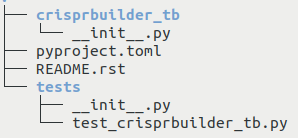
\includegraphics[width=6cm]{nom_package_tree.png}

Le fichier \textit{nom\_package.toml} remplace les anciens standards de définition de packages : \textit{setup.exe} et \textit{requirements.txt}. Il précise notamment le nom du package, sa version, sa description, l’emplacement de son dépôt (par exemple sur GitHub), l’adresse email de l’auteur du package, et la version des dépendances.

En ce qui concerne la version des dépendances, il faut tout d'abord se placer dans le répertoire \textit{nom\_package} puis utiliser l’instruction
\begin{tcolorbox}\texttt{poetry add nom\_dependance}\end{tcolorbox}  
qui assure la compatibilité de la dépendance \textit{nom\_dependance} avec le package \textit{nom\_package}. Il est également possible d’imposer certaines contraintes sur les versions des dépendances ou encore de rentrer manuellement les dépendances dans le fichier \textit{nom\_package.toml}, mais l’instruction 
\begin{tcolorbox}\texttt{poetry add nom\_dependance}\end{tcolorbox}  
offre l’avantage de chercher automatiquement une version compatible de la dépendance, puis de l’inscrire dans \textit{nom\_package.toml}.

Pour installer ensuite les dépendances du projet, il est nécessaire d’utiliser l’instruction
\begin{tcolorbox}\texttt{poetry install}\end{tcolorbox}
qui crée le fichier \textit{mon\_package.lock}. Ce fichier empêche les dépendances de télécharger la dernière version au moment de l’installation, en fixant la version utilisable par le package.


% CONSTRUCTION D'UN PACKAGE -------------------
\subsection{Construction d'un package et publication}

Pour empaqueter le projet, il faut utiliser l’instruction
\begin{tcolorbox}\texttt{poetry build}\end{tcolorbox}
qui va permettre de créer un fichier source au format \textit{sdist} et une distribution compilée au format \textit{wheel}.

On peut vérifier la conformité du package avec l’instruction
\begin{tcolorbox}\texttt{poetry check}\end{tcolorbox}
qui renvoie
\begin{tcolorbox}\texttt{All set !}\end{tcolorbox}
si le package ne comporte aucune discordance et peut être publié.

Avant de publier le package, il peut être bon de tester son comportement à l'installation. Pour cela, il est possible de le publier officieusement sur la plateforme de test \textit{testPyPI}. Il faut alors se placer à la racine du package et lancer en ligne de commande l'instruction
\begin{tcolorbox}\texttt{twine upload --repository testpypi dist/*}\end{tcolorbox}

L'installation du package à partir de \textit{testPyPI} se fait à l'aide de l'instruction
\begin{tcolorbox}\texttt{pip3 install -i https://test.pypi.org/simple/ nom\_package}\end{tcolorbox} ou si on précise la version du package
\begin{tcolorbox}\texttt{pip3 install -i https://test.pypi.org/simple/ nom\_package==nmr\_version}\end{tcolorbox} A noter qu'il ne faut utiliser de guillemets autour de la version du package.

Lorsque le package est finalement prêt pour être publié sur PyPI, on utilise l’instruction
\begin{tcolorbox}\texttt{poetry publish}\end{tcolorbox}
L'auteur du package doit pour cela être enregistré sur PyPI avec un identifiant et un mot de passe. A partir de ce moment-là, le package est rendu disponible publiquement.

L’installation du package par un utilisateur quelconque se fait maintenant grâce à l’instruction
\begin{tcolorbox}\texttt{python3 -m pip install nom\_package}\end{tcolorbox}

Les explications relatives à l’utilisation pratique de \textit{Poetry} sont reprises dans le tutoriel suivant que nous venons de publier sur YouTube : adresse YuouTube



% CONSTRUCTION DU PACKAGE CRISPR -----------------
\subsection{La construction du package crisprbuilder\_tb}

Par exemple pour construire le package \textit{crisprbuilder\_tb} à l'aide de \textit{Poetry}, les instructions suivantes sont nécessaires en ligne de commande :

\begin{tcolorbox}\texttt{poetry new crisprbuilder\_tb
cd crisprbuilder\_tb \\
poetry add python3 \\
poetry add xlrd \\
poetry add xmltodict \\
poetry add biopython \\
poetry install \\
poetry build \\
poetry check \\
poetry publish}\end{tcolorbox}


	% LA COMPOSITION DU PACKAGE ------------------------
	
	\section{La composition du package}

Le package est décrit en détail dans le document crisprbuilder\_tb.md


Ainsi, une recherche effectuée à partir de ERR2704808 permet d'obtenir le résultat suivant :


% LA STRUCTURE D'UN PACKAGE SOUS POETRY
\section{La structure d'un package sous Poetry}

Lors de l'exécution de l'instruction poetry new crisprbuilder\_tb s'est créé le package crisprbuilder\_tb disposant de la structure suivante :

photo structure

Le répertoire crisprbuilder\_tb contient les fichiers \_\_init\_\_.py et \_\_main\_\_.py





% PYLINT --------------
\section{Améliorer le code avec pylint}

\textit{pylint} fournit une note entre 0 et 10 qui reflète le respect des règles du PEP8, notamment en ce qui concerne la lisibilité du code. Il reprend également certaines exigences relatives à ...

Le fichier \textit{\_\_main\_\_.py} est noté 9, / 10 avec les commentaires suivants :
XXX

et le fichier \textit{support.py} est noté 9, / 10 avec les commentaires suivants :
XXX

S'agissant d'un test statique, le code n'est pas exécuté et la performance du code n'est pas prise en compte lors de l'évaluation faite par \textit{pylint}. Ainsi, \textit{pylint} peut reprocher l'utilisation injustifiée de listes compréhensives, sans tenir compte de l'efficacité d'un tel traitement.


% DESCRIPTION DU PACKAGE ---------------------------
\section{Description du package avec le fichier crisprbuilder\_tb.md}



% CREATION DE LA LIBRAIRIE --------------------------------

\section{La création de la librairie}

=== A CHANGER ===
Pour créer une librairie à partir de conda, il est nécessaire d'installer conda-build puis de construire un recipe composé de :
\begin{itemize}
\item un fichier meta.yaml contenant toutes les métadata du recipe
\item un script build.sh qui installe les fichiers de la librairie sur Linux et macOS, exécuté avec une commande bash
\item un script bld.bat qui installe les fichiers de la librairie sur Windows, exécuté avec une commande cmd
\item un fichier optionnel $run_test.py$, qui s'exécute automatiquement pour effectuer des tests
\item un fichier readme et des icônes si nécessaire.  
\end{itemize}
Les trois premiers fichiers se créent avec la commande conda skeleton.
===FIN CHANGEMENT===



% LES TESTS DU PACKAGE -----------------------
\chapter{Les tests du package}





% AMELIORATION DES PERFORMANCES -----------------------
\chapter{Amélioration des performances}


% CONCLUSION ----------------------
\chapter*{Conclusion}

Ce stage m'a ouvert l'esprit vers le domaine de la bioinformatique et m'a permis de réfléchir à 

	
	
PROBLEME

mv /home/stephane/.local/lib/python3.6/site-packages/crisprtest /home/stephane/Téléchargements

répétition de pip install
	

% LES ELEMENTS DU CODE ------------------------------------------

\section{Les principaux éléments du code}

dico est composé de la façon suivante :

Un fichier pkl tel que dico\_africanum.pkl est créé par pickle et contient un flux d'octets représentant les objets à sérialiser.

pickle permet aux objets d'être sérialisés en fichiers sur disque et désérialisés dans le programme au moment de l'exécution.
	
	% =========
	% BIBLIOTHEQUE
	% =========
	\begin{spacing}{0.5}
		\bibliographystyle{}
		\renewcommand{\bibname}{Références}
		\begin{thebibliography}{10}
			\href{https://packaging.python.org/guides/}{https://packaging.python.org/guides/}\\

\href{https://realpython.com/pypi-publish-python-package/}{https://realpython.com/pypi-publish-python-package/}
			
		\end{thebibliography}
	\end{spacing}



% INDEX ------------------
\printindex




\end{document}
